\documentclass[fleqn, a4paper, 12pt, russian]{article}

\usepackage[utf8]{inputenc}
\usepackage[T1, T2A]{fontenc}
\usepackage[english, main = russian]{babel}
\usepackage{indentfirst}
\usepackage{graphicx}
\usepackage{natbib}
\usepackage{amsmath}
\usepackage{pdflscape}
\usepackage{caption, subcaption}
\graphicspath{{../imgs/}}

\captionsetup[figure]{name = Рисунок, labelsep = endash}
\captionsetup[table]{name = Таблица, labelsep = endash, justification=raggedright, singlelinecheck=false}
\setlength{\mathindent}{0pt}

\begin{document}

	\begin{center}
		\begin{tabular}{|c|c|}
			\hline
			Параметр & Описание \\ \hline
			$\alpha(t)$& угол поворота тележки\\ \hline
			$x(t),y(t)$& координаты цетра тележки в абсолютной системе координат\\ \hline
			$q$ & вектор обобщённых координат тележки\\ \hline
			$A(q)$ & матрица преобразования из абсолютной СК в СК тележки\\ \hline
			$R$ & радиус-вектор центра тележки в абсолютной СК\\ \hline
			$K$ & кинетическая энергия системы\\ \hline
			$L$ & лагранжиан системы\\ \hline
			$\tau$ & вектор обобщённых сил, действующих на тележку \\ \hline
			$l$ & расстояние от центра тележки до колеса по оси Oy\\ \hline
			$r$ & радиус колёс тележки \\ \hline
			$\tau_1, \tau_2$ & моменты, развиваемые на колёсах тележки \\ \hline
			$T,F_1, F_2$ & момент и силы, действующие на тележку \\ \hline
			$E$& матрица согласования $\tau_1, \tau_2$ с 	$T,F_1, F_2$ \\ \hline
			
		\end{tabular}
	\end{center}

	Выделим две системы координат: абсолютная СК, начало которой совпадает с краем рабочей области и СК тележки, начало которой находится в центре тележки.
	
	Пусть угол поворота тележки, т.е. угол поворота между указанными двумя СК равен $\alpha(t)$, а координаты тележки равны $(x(t),y(t))$, обозначим вектор обобщённых координат тележки за $q(t) = [\alpha(t)~x(t)~y(t)]^T=q$. тогда указанные системы координат будут связаны следующей матрицей преобразования: 
	
	
	
	\begin{equation}
		A(q)=\begin{bmatrix}
		\cos(\alpha(t)) & -\sin(\alpha(t)) &x(t)\\
		\sin(\alpha(t)) &  \cos(\alpha(t)) & y(t)\\
		0    &     0 &         1  \\
		\end{bmatrix}
	\end{equation}
	
	Пусть центр тяжести в СК тележки имеет координаты $(c_x,c_y)$.	Тогда центр масс тележки будет иметь в базовой СК следующие координаты:
	
	\begin{equation}
		R = A(q)\begin{bmatrix}
			c_x\\c_y\\1
		\end{bmatrix}=\begin{bmatrix}
			c_x\cos(\alpha(t))-	c_y\sin(\alpha(t)) +x(t)\\
			c_x\sin(\alpha(t))+	c_y\cos(\alpha(t)) +y(t)\\
			1
		\end{bmatrix}
	\end{equation}
	
	При таком алгоритме подсчёта $R$ расширяется до размерности 3х1. Нам нужны только первые две координаты, но т.к. при подсчёте кинетической энергии нам нужен квадрат производной, а третья координата $R_3\equiv 1$, то $\dot{R_3}\equiv 0$, что при возведении вектора $\dot{R}$ в квадрат $\dot{R}^T*\dot{R}$ не привнесёт никаких изменений. Поэтому не будем тратить время на редуцирование вектора $R$, а будем дальше использовать его таким, как он есть.
	
	
	Т.к. потенциальна энергия постоянна (тележка всегда находится на одной высоте), то Лагранжиан системы $L = K - H$, где $K$ - кинетическая, $H$ -  потенциальная энергия, принимает вид $L=K$.
	
	\begin{equation}
		L = K = \frac{1}{2}(m\dot{R}^T\dot{R}+I\dot{\alpha}^2)
	\end{equation} 
	
	
	\begin{equation}
		 \frac{\partial }{\partial t}R = \frac{\partial }{\partial t} (A(q)*[c_x~c_y~1]^T)=
		\begin{bmatrix}
			\dot{x(t)} - c_y\cos(\alpha(t))\dot{\alpha(t)} - c_x\sin(\alpha(t))\dot{\alpha(t)}\\
			\dot{y(t)} + c_x\cos(\alpha(t))\dot{\alpha(t)} - c_y\sin(\alpha(t))\dot{\alpha(t)}\\
			0\\
		\end{bmatrix}
	\end{equation}
	
	После группировки:
	
	\begin{equation}
	 \frac{\partial }{\partial t}R =
	\begin{bmatrix}
	\dot{x(t)} - \dot{\alpha(t)}(c_y\cos(\alpha(t))+ c_x\sin(\alpha(t)))\\
	\dot{y(t)} - \dot{\alpha(t)}(c_y\sin(\alpha(t))- c_x\cos(\alpha(t)))\\
	0\\
	\end{bmatrix}
	\end{equation}

Тогда 

$\dot{R}^T\dot{R} = (\dot{x(t)} - \dot{\alpha(t)}(c_y\cos(\alpha(t))+ c_x\sin(\alpha(t))))^2+(\dot{y(t)} - \dot{\alpha(t)}(c_y\sin(\alpha(t))- c_x\cos(\alpha(t))))^2$

Раскроем скобки:

$\dot{R}^T\dot{R} = \dot{x(t)}^2+\dot{\alpha(t)}^2(c_y\cos(\alpha(t))+ c_x\sin(\alpha(t)))^2-2\dot{x(t)}\dot{\alpha(t)}(c_y\cos(\alpha(t))+ c_x\sin(\alpha(t)))+\dot{y(t)}^2+\dot{\alpha(t)}^2(c_y\sin(\alpha(t))- c_x\cos(\alpha(t)))^2-2\dot{y(t)}\dot{\alpha(t)}(c_y\sin(\alpha(t))- c_x\cos(\alpha(t)))$
	
Сгруппируем слагаемые:
	
$\dot{R}^T\dot{R} = \dot{x(t)}^2+\dot{y(t)}^2 + \dot{\alpha(t)}^2( (c_y\cos(\alpha(t))+ c_x\sin(\alpha(t)))^2+(c_y\sin(\alpha(t))- c_x\cos(\alpha(t)))^2) -2\dot{\alpha(t)}(\dot{x(t)}(c_y\cos(\alpha(t))+ c_x\sin(\alpha(t)))+\dot{y(t)}(c_y\sin(\alpha(t))- c_x\cos(\alpha(t))))$
	
В слагаемом при $\dot{\alpha(t)}^2$ несложно увидеть основное тригонометрическое тождество при раскрытии скобок:

$(c_y\cos(\alpha(t))+ c_x\sin(\alpha(t)))^2+(c_y\sin(\alpha(t))- c_x\cos(\alpha(t)))^2=c_y^2+c_x^2$

Тогда исходное выражение можно представить в следующем виде:

$\dot{R}^T\dot{R} = \dot{x(t)}^2+\dot{y(t)}^2 + \dot{\alpha(t)}^2(c_y^2+c_x^2) -2\dot{\alpha(t)}(\dot{x(t)}c_y\cos(\alpha(t))+ \dot{x(t)}c_x\sin(\alpha(t))+\dot{y(t)}c_y\sin(\alpha(t))- \dot{y(t)}c_x\cos(\alpha(t)))$

Найдём отдельно производную $\dot{R}^T\dot{R}$ по $q$:


$\frac{\partial (\dot{R}^T\dot{R})}{\partial q} = 
-2\dot{\alpha(t)}\begin{bmatrix}
-\dot{x(t)}c_y\sin(\alpha(t))+\dot{x(t)}c_x\cos(\alpha(t))+\dot{y(t)}c_y\cos(\alpha(t)+ \dot{y(t)}c_x\sin(\alpha(t))\\0\\0
\end{bmatrix}
$


Тогда 

\begin{equation*}
\frac{\partial K}{\partial q}= -m\dot{\alpha(t)}\begin{bmatrix}
\dot{x(t)}c_x\cos(\alpha(t))-\dot{x(t)}c_y\sin(\alpha(t))+\dot{y(t)}c_y\cos(\alpha(t))+ \dot{y(t)}c_x\sin(\alpha(t))\\0\\0
\end{bmatrix}
\end{equation*}


Теперь найдём отдельно производную $\dot{R}^T\dot{R}$ по $\dot{q}$:

$\scriptsize{\frac{\partial (\dot{R}^T\dot{R})}{\partial \dot{q}} = 
	\begin{bmatrix}
	2\dot{\alpha(t)}(c_y^2+c_x^2)-2(\dot{x(t)}c_y\cos(\alpha(t))+ \dot{x(t)}c_x\sin(\alpha(t))+\dot{y(t)}c_y\sin(\alpha(t))- \dot{y(t)}c_x\cos(\alpha(t)))\\	 
	2\dot{x(t)}-2\dot{\alpha(t)}(c_y\cos(\alpha(t))+ c_x\sin(\alpha(t)))\\	  
	2\dot{y(t)}-2{\alpha(t)}(c_y\sin(\alpha(t))- c_x\cos(\alpha(t)))	 
	\end{bmatrix}}$



$\scriptsize{\frac{\partial (\dot{R}^T\dot{R})}{\partial \dot{q}} = 
2\begin{bmatrix}
	 \dot{\alpha(t)}(c_y^2+c_x^2)-\dot{x(t)}c_y\cos(\alpha(t))-\dot{x(t)}c_x\sin(\alpha(t))-\dot{y(t)}c_y\sin(\alpha(t))+ \dot{y(t)}c_x\cos(\alpha(t))\\	 
	 \dot{x(t)}-\dot{\alpha(t)}(c_y\cos(\alpha(t))+ c_x\sin(\alpha(t)))\\	  
	  \dot{y(t)}-\dot{\alpha(t)}(c_y\sin(\alpha(t))- c_x\cos(\alpha(t)))	 
\end{bmatrix}}$


$\scriptsize{\frac{\partial }{\partial t}\frac{\partial (\dot{R}^T\dot{R})}{\partial \dot{q}} = 
	2\frac{\partial }{\partial t}\begin{bmatrix}
 \dot{\alpha(t)}(c_y^2+c_x^2)-(\dot{x(t)}c_y\cos(\alpha(t))+ \dot{x(t)}c_x\sin(\alpha(t))+\dot{y(t)}c_y\sin(\alpha(t))- \dot{y(t)}c_x\cos(\alpha(t)))\\	 
\dot{x(t)}-\dot{\alpha(t)}(c_y\cos(\alpha(t))+ c_x\sin(\alpha(t)))\\	  
\dot{y(t)}-\dot{\alpha(t)}(c_y\sin(\alpha(t))- c_x\cos(\alpha(t)))	 
	\end{bmatrix}}$

Найдём для начала промежуточные значения выражений

$\frac{\partial }{\partial t}(\dot{\alpha(t)}(c_y^2+c_x^2)-\dot{x(t)}c_y\cos(\alpha(t))- \dot{x(t)}c_x\sin(\alpha(t))-\dot{y(t)}c_y\sin(\alpha(t))+ \dot{y(t)}c_x\cos(\alpha(t))))
=\ddot{\alpha(t)}(c_y^2+c_x^2)-
\ddot{x(t)}c_y\cos(\alpha(t))+\dot{x(t)}\dot{\alpha(t)}c_y\sin(\alpha(t))+ 
\ddot{x(t)}c_x\sin(\alpha(t))+\dot{x(t)}\dot{\alpha(t)}c_x\cos(\alpha(t))-
\ddot{y(t)}c_y\sin(\alpha(t))-\dot{y(t)}\dot{\alpha(t)}c_y\cos(\alpha(t))+ 
\ddot{y(t)}c_x\cos(\alpha(t))-\dot{y(t)}\dot{\alpha(t)}c_x\sin(\alpha(t))
$

$\frac{\partial }{\partial t}(\dot{x(t)}-\dot{\alpha(t)}(c_y\cos(\alpha(t))+ c_x\sin(\alpha(t)))) = 
\ddot{x(t)}
-\ddot{\alpha(t)}(c_y\cos(\alpha(t))+ c_x\sin(\alpha(t)))-\dot{\alpha(t)}(-\dot{\alpha(t)}c_y\sin(\alpha(t))+ \dot{\alpha(t)}c_x\cos(\alpha(t)))
$

$\frac{\partial }{\partial t}(\dot{y(t)}-\dot{\alpha(t)}(c_y\sin(\alpha(t))- c_x\cos(\alpha(t))))=
\ddot{y(t)}
-\ddot{\alpha(t)}(c_y\sin(\alpha(t))- c_x\cos(\alpha(t)))-\dot{\alpha(t)}(\dot{\alpha(t)}c_y\cos(\alpha(t))+ \dot{\alpha(t)}c_x\sin(\alpha(t)))
$



$\scriptsize{\frac{\partial }{\partial t}\frac{\partial (\dot{R}^T\dot{R})}{\partial \dot{q}} = 
	2\begin{bmatrix}
	\dot{x(t)}\dot{\alpha(t)}c_y\sin(\alpha(t))
	+\dot{x(t)}\dot{\alpha(t)}c_x\cos(\alpha(t))
	-\dot{y(t)}\dot{\alpha(t)}c_y\cos(\alpha(t))
	-\dot{y(t)}\dot{\alpha(t)}c_x\sin(\alpha(t))\\
	-\dot{\alpha(t)}(-\dot{\alpha(t)}c_y\sin(\alpha(t))+ \dot{\alpha(t)}c_x\cos(\alpha(t)))\\
	-\dot{\alpha(t)}(\dot{\alpha(t)}c_y\cos(\alpha(t))+ \dot{\alpha(t)}c_x\sin(\alpha(t)))
	\end{bmatrix}}+$
	
	$\scriptsize{2\begin{bmatrix}
		\ddot{\alpha(t)}(c_y^2+c_x^2)-
		\ddot{x(t)}c_y\cos(\alpha(t))+ 
		\ddot{x(t)}c_x\sin(\alpha(t))-
		\ddot{y(t)}c_y\sin(\alpha(t))+ 
		\ddot{y(t)}c_x\cos(\alpha(t))\\
			\ddot{x(t)}
		-\ddot{\alpha(t)}(c_y\cos(\alpha(t))+ c_x\sin(\alpha(t)))\\
			\ddot{y(t)}
		-\ddot{\alpha(t)}(c_y\sin(\alpha(t))- c_x\cos(\alpha(t)))
		\end{bmatrix}}$
		

$\scriptsize{\frac{\partial }{\partial t}\frac{\partial K}{\partial \dot{q}} = 
	m\begin{bmatrix}
	\dot{x(t)}\dot{\alpha(t)}c_y\sin(\alpha(t))
	+\dot{x(t)}\dot{\alpha(t)}c_x\cos(\alpha(t))
	-\dot{y(t)}\dot{\alpha(t)}c_y\cos(\alpha(t))
	-\dot{y(t)}\dot{\alpha(t)}c_x\sin(\alpha(t))\\
	-\dot{\alpha(t)}(-\dot{\alpha(t)}c_y\sin(\alpha(t))+ \dot{\alpha(t)}c_x\cos(\alpha(t)))\\
	- c_x\cos(\alpha(t)))-\dot{\alpha(t)}(\dot{\alpha(t)}c_y\cos(\alpha(t))+ \dot{\alpha(t)}c_x\sin(\alpha(t)))
	\end{bmatrix}}+$

$\scriptsize{m\begin{bmatrix}
	\ddot{\alpha(t)}(c_y^2+c_x^2)-
	\ddot{x(t)}c_y\cos(\alpha(t))+ 
	\ddot{x(t)}c_x\sin(\alpha(t))-
	\ddot{y(t)}c_y\sin(\alpha(t))+ 
	\ddot{y(t)}c_x\cos(\alpha(t))\\
	\ddot{x(t)}
	-\ddot{\alpha(t)}(c_y\cos(\alpha(t))+ c_x\sin(\alpha(t)))\\
	\ddot{y(t)}
	-\ddot{\alpha(t)}(c_y\sin(\alpha(t))- c_x\cos(\alpha(t)))
	\end{bmatrix}+\begin{bmatrix}
I\ddot{\alpha(t)}\\0\\0
\end{bmatrix}}$

\newpage

Итоговое динамическое уравнение тележки можно представить как:

$\scriptsize{\frac{\partial K}{\partial q} - \frac{\partial }{\partial t}\frac{\partial K}{\partial \dot{q}}=
m\dot{\alpha(t)}\begin{bmatrix}
\dot{x(t)}c_x\cos(\alpha(t))-\dot{x(t)}c_y\sin(\alpha(t))+\dot{y(t)}c_y\cos(\alpha(t))+ \dot{y(t)}c_x\sin(\alpha(t))\\0\\0
\end{bmatrix}}+$

$\scriptsize{m\begin{bmatrix}
	\dot{x(t)}\dot{\alpha(t)}c_y\sin(\alpha(t))
	+\dot{x(t)}\dot{\alpha(t)}c_x\cos(\alpha(t))
	-\dot{y(t)}\dot{\alpha(t)}c_y\cos(\alpha(t))
	-\dot{y(t)}\dot{\alpha(t)}c_x\sin(\alpha(t))\\
	-\dot{\alpha(t)}^2(c_x\cos(\alpha(t))-c_y\sin(\alpha(t)))\\
	-\dot{\alpha(t)}^2(c_x\sin(\alpha(t))+c_y\cos(\alpha(t)))
	\end{bmatrix}}+
$

$\scriptsize{m\begin{bmatrix}
	\ddot{\alpha(t)}(c_y^2+c_x^2)-
	\ddot{x(t)}c_y\cos(\alpha(t))+ 
	\ddot{x(t)}c_x\sin(\alpha(t))-
	\ddot{y(t)}c_y\sin(\alpha(t))+ 
	\ddot{y(t)}c_x\cos(\alpha(t))\\
	\ddot{x(t)}
	-\ddot{\alpha(t)}(c_y\cos(\alpha(t))+ c_x\sin(\alpha(t)))\\
	\ddot{y(t)}
	-\ddot{\alpha(t)}(c_y\sin(\alpha(t))- c_x\cos(\alpha(t)))
	\end{bmatrix}-\begin{bmatrix}
	I\ddot{\alpha(t)}\\0\\0
	\end{bmatrix}}$


Представим уравнение динамики тележки в форме:

\begin{equation}
	M(q)\ddot{q}+C(q,\dot{q})\dot{q}+G(q)=\tau
\end{equation}


$\scriptsize{M(q)=\begin{bmatrix} 
	m(c_x^2+c_y^2)-I& m(c_x\sin(\alpha(t))-c_y\cos(\alpha(t)))&m(c_x\cos(\alpha(t))-c_y\sin(\alpha(t)))\\
	m(-c_x\sin(\alpha(t))-c_y\cos(\alpha(t)))&m&0\\
	m(c_x\cos(\alpha(t))-c_y\sin(\alpha(t)))&0&m\\
\end{bmatrix}}$

$\scriptsize{C=m\begin{bmatrix}
	0&c_x\cos(\alpha(t))-c_y\sin(\alpha(t))&c_x\sin(\alpha(t))+c_y\cos(\alpha(t))\\	
	0&0&0\\
	0&0&0
\end{bmatrix}}$

$\scriptsize{+m\begin{bmatrix}
		0&\dot{\alpha(t)}(c_x\cos(\alpha(t))+c_y\sin(\alpha(t)))&-\dot{\alpha(t)}(-c_x\sin(\alpha(t))-c_y\cos(\alpha(t)))\\	
		\dot{\alpha(t)}(-c_x\cos(\alpha(t))+c_y\sin(\alpha(t)))&0&0\\
		-\dot{\alpha(t)}(c_x\sin(\alpha(t))+c_y\cos(\alpha(t)))&0&0
\end{bmatrix}}$


$\tiny{C=m\begin{bmatrix}
	0&(\dot{\alpha(t)}+1)c_x\cos(\alpha(t))+(\dot{\alpha(t)}-1)c_y\sin(\alpha(t))&
	(\dot{\alpha(t)}+1)(c_x\sin(\alpha(t))+c_y\cos(\alpha(t)))\\
	\dot{\alpha(t)}(c_y\sin(\alpha(t))-c_x\cos(\alpha(t)))&0&0\\
	-\dot{\alpha(t)}(c_x\sin(\alpha(t))+c_y\cos(\alpha(t)))&0&0
\end{bmatrix}}$

$G=\begin{bmatrix} 0\\ 0\\ 0 \end{bmatrix}$

Для моделирования поведения системы, введём переменную состояния $X=[q^T~\dot{q}^T]^T$.
Тогда исходное уравнение динамики можно свести к аффинной системе вида $\dot{X}=f(X)+g(X)\tau$:

$f(X) = \begin{bmatrix}
	0_{3x3} &I_{3x3}\\
	0_{3x3} & M(q)^{-1}C(q,\dot{q})
\end{bmatrix}X$

$g(X) = \begin{bmatrix}
	0_{3x3}\\
	M(q)^{-1}
\end{bmatrix}$


\newpage
$\tiny{M=
\left(\begin{array}{ccc} m\,\left({\mathrm{cx}}^2+{\mathrm{cy}}^2\right)-I & -m\,\left(\mathrm{cy}\,\cos\left(\mathrm{at}\right)-\mathrm{cx}\,\sin\left(\mathrm{at}\right)\right) & m\,\left(\mathrm{cx}\,\cos\left(\mathrm{at}\right)-\mathrm{cy}\,\sin\left(\mathrm{at}\right)\right)\\ -m\,\left(\mathrm{cy}\,\cos\left(\mathrm{at}\right)+\mathrm{cx}\,\sin\left(\mathrm{at}\right)\right) & m & 0\\ m\,\left(\mathrm{cx}\,\cos\left(\mathrm{at}\right)-\mathrm{cy}\,\sin\left(\mathrm{at}\right)\right) & 0 & m \end{array}\right)
}$

$\tiny{
C=
\left(\begin{array}{ccc} 0 & \mathrm{cx}\,\cos\left(\mathrm{at}\right)\,\left(\mathrm{dat}+1\right)+\mathrm{cy}\,\sin\left(\mathrm{at}\right)\,\left(\mathrm{dat}-1\right) & \left(\mathrm{cy}\,\cos\left(\mathrm{at}\right)+\mathrm{cx}\,\sin\left(\mathrm{at}\right)\right)\,\left(\mathrm{dat}+1\right)\\ -\mathrm{dat}\,\left(\mathrm{cx}\,\cos\left(\mathrm{at}\right)-\mathrm{cy}\,\sin\left(\mathrm{at}\right)\right) & 0 & 0\\ -\mathrm{dat}\,\left(\mathrm{cy}\,\cos\left(\mathrm{at}\right)+\mathrm{cx}\,\sin\left(\mathrm{at}\right)\right) & 0 & 0 \end{array}\right)
}$

\begin{landscape}
$\tiny{M(q)^{-1}=
	\left(\begin{array}{ccc} -\frac{1}{I-{\mathrm{cx}}^2\,m+{\mathrm{cx}}^2\,m\,\cos\left(2\,\mathrm{at}\right)-\mathrm{cx}\,\mathrm{cy}\,m\,\sin\left(2\,\mathrm{at}\right)} & -\frac{\mathrm{cy}\,\cos\left(\mathrm{at}\right)-\mathrm{cx}\,\sin\left(\mathrm{at}\right)}{2\,m\,{\mathrm{cx}}^2\,{\cos\left(\mathrm{at}\right)}^2-2\,m\,{\mathrm{cx}}^2-2\,\mathrm{cy}\,m\,\sin\left(\mathrm{at}\right)\,\mathrm{cx}\,\cos\left(\mathrm{at}\right)+I} & \frac{\mathrm{cx}\,\cos\left(\mathrm{at}\right)-\mathrm{cy}\,\sin\left(\mathrm{at}\right)}{2\,m\,{\mathrm{cx}}^2\,{\cos\left(\mathrm{at}\right)}^2-2\,m\,{\mathrm{cx}}^2-2\,\mathrm{cy}\,m\,\sin\left(\mathrm{at}\right)\,\mathrm{cx}\,\cos\left(\mathrm{at}\right)+I}\\ -\frac{\mathrm{cy}\,\cos\left(\mathrm{at}\right)+\mathrm{cx}\,\sin\left(\mathrm{at}\right)}{2\,m\,{\mathrm{cx}}^2\,{\cos\left(\mathrm{at}\right)}^2-2\,m\,{\mathrm{cx}}^2-2\,\mathrm{cy}\,m\,\sin\left(\mathrm{at}\right)\,\mathrm{cx}\,\cos\left(\mathrm{at}\right)+I} & -\frac{{\mathrm{cx}}^2\,m-2\,I+{\mathrm{cy}}^2\,m-{\mathrm{cx}}^2\,m\,\cos\left(2\,\mathrm{at}\right)+{\mathrm{cy}}^2\,m\,\cos\left(2\,\mathrm{at}\right)+2\,\mathrm{cx}\,\mathrm{cy}\,m\,\sin\left(2\,\mathrm{at}\right)}{2\,m\,\left(I-{\mathrm{cx}}^2\,m+{\mathrm{cx}}^2\,m\,\cos\left(2\,\mathrm{at}\right)-\mathrm{cx}\,\mathrm{cy}\,m\,\sin\left(2\,\mathrm{at}\right)\right)} & \frac{\frac{\sin\left(2\,\mathrm{at}\right)\,{\mathrm{cx}}^2}{2}+\cos\left(2\,\mathrm{at}\right)\,\mathrm{cx}\,\mathrm{cy}-\frac{\sin\left(2\,\mathrm{at}\right)\,{\mathrm{cy}}^2}{2}}{I-{\mathrm{cx}}^2\,m+{\mathrm{cx}}^2\,m\,\cos\left(2\,\mathrm{at}\right)-\mathrm{cx}\,\mathrm{cy}\,m\,\sin\left(2\,\mathrm{at}\right)}\\ \frac{\mathrm{cx}\,\cos\left(\mathrm{at}\right)-\mathrm{cy}\,\sin\left(\mathrm{at}\right)}{2\,m\,{\mathrm{cx}}^2\,{\cos\left(\mathrm{at}\right)}^2-2\,m\,{\mathrm{cx}}^2-2\,\mathrm{cy}\,m\,\sin\left(\mathrm{at}\right)\,\mathrm{cx}\,\cos\left(\mathrm{at}\right)+I} & -\frac{\frac{\sin\left(2\,\mathrm{at}\right)\,{\mathrm{cx}}^2}{2}-\mathrm{cx}\,\mathrm{cy}+\frac{\sin\left(2\,\mathrm{at}\right)\,{\mathrm{cy}}^2}{2}}{I-{\mathrm{cx}}^2\,m+{\mathrm{cx}}^2\,m\,\cos\left(2\,\mathrm{at}\right)-\mathrm{cx}\,\mathrm{cy}\,m\,\sin\left(2\,\mathrm{at}\right)} & \frac{2\,I-3\,{\mathrm{cx}}^2\,m-{\mathrm{cy}}^2\,m+{\mathrm{cx}}^2\,m\,\cos\left(2\,\mathrm{at}\right)+{\mathrm{cy}}^2\,m\,\cos\left(2\,\mathrm{at}\right)}{2\,m\,\left(I-{\mathrm{cx}}^2\,m+{\mathrm{cx}}^2\,m\,\cos\left(2\,\mathrm{at}\right)-\mathrm{cx}\,\mathrm{cy}\,m\,\sin\left(2\,\mathrm{at}\right)\right)} \end{array}\right)
}$

$\tiny{
	inv(curM)*curC=
	\left(\begin{array}{ccc} -\frac{\mathrm{cx}\,\mathrm{dat}\,\left(\mathrm{cy}\,\cos\left(2\,\mathrm{at}\right)-\mathrm{cy}+\mathrm{cx}\,\sin\left(2\,\mathrm{at}\right)\right)}{I-{\mathrm{cx}}^2\,m+{\mathrm{cx}}^2\,m\,\cos\left(2\,\mathrm{at}\right)-\mathrm{cx}\,\mathrm{cy}\,m\,\sin\left(2\,\mathrm{at}\right)} & -\frac{\mathrm{cx}\,\cos\left(\mathrm{at}\right)-\mathrm{cy}\,\sin\left(\mathrm{at}\right)+\mathrm{cx}\,\mathrm{dat}\,\cos\left(\mathrm{at}\right)+\mathrm{cy}\,\mathrm{dat}\,\sin\left(\mathrm{at}\right)}{2\,m\,{\mathrm{cx}}^2\,{\cos\left(\mathrm{at}\right)}^2-2\,m\,{\mathrm{cx}}^2-2\,\mathrm{cy}\,m\,\sin\left(\mathrm{at}\right)\,\mathrm{cx}\,\cos\left(\mathrm{at}\right)+I} & -\frac{\left(\mathrm{cy}\,\cos\left(\mathrm{at}\right)+\mathrm{cx}\,\sin\left(\mathrm{at}\right)\right)\,\left(\mathrm{dat}+1\right)}{2\,m\,{\mathrm{cx}}^2\,{\cos\left(\mathrm{at}\right)}^2-2\,m\,{\mathrm{cx}}^2-2\,\mathrm{cy}\,m\,\sin\left(\mathrm{at}\right)\,\mathrm{cx}\,\cos\left(\mathrm{at}\right)+I}\\ -\frac{I\,\mathrm{dat}\,\left(\mathrm{cx}\,\cos\left(\mathrm{at}\right)-\mathrm{cy}\,\sin\left(\mathrm{at}\right)\right)}{m\,\left(2\,m\,{\mathrm{cx}}^2\,{\cos\left(\mathrm{at}\right)}^2-2\,m\,{\mathrm{cx}}^2-2\,\mathrm{cy}\,m\,\sin\left(\mathrm{at}\right)\,\mathrm{cx}\,\cos\left(\mathrm{at}\right)+I\right)} & -\frac{\frac{{\mathrm{cx}}^2\,\sin\left(2\,\mathrm{at}\right)}{2}-\frac{{\mathrm{cy}}^2\,\sin\left(2\,\mathrm{at}\right)}{2}+\mathrm{cx}\,\mathrm{cy}\,\cos\left(2\,\mathrm{at}\right)+\mathrm{cx}\,\mathrm{cy}\,\mathrm{dat}+\frac{{\mathrm{cx}}^2\,\mathrm{dat}\,\sin\left(2\,\mathrm{at}\right)}{2}+\frac{{\mathrm{cy}}^2\,\mathrm{dat}\,\sin\left(2\,\mathrm{at}\right)}{2}}{I-{\mathrm{cx}}^2\,m+{\mathrm{cx}}^2\,m\,\cos\left(2\,\mathrm{at}\right)-\mathrm{cx}\,\mathrm{cy}\,m\,\sin\left(2\,\mathrm{at}\right)} & -\frac{\left(\mathrm{dat}+1\right)\,\left(\frac{{\mathrm{cy}}^2\,\cos\left(2\,\mathrm{at}\right)}{2}-\frac{{\mathrm{cx}}^2\,\cos\left(2\,\mathrm{at}\right)}{2}+\frac{{\mathrm{cx}}^2}{2}+\frac{{\mathrm{cy}}^2}{2}+\mathrm{cx}\,\mathrm{cy}\,\sin\left(2\,\mathrm{at}\right)\right)}{I-{\mathrm{cx}}^2\,m+{\mathrm{cx}}^2\,m\,\cos\left(2\,\mathrm{at}\right)-\mathrm{cx}\,\mathrm{cy}\,m\,\sin\left(2\,\mathrm{at}\right)}\\ \frac{\mathrm{dat}\,\left(2\,m\,\sin\left(\mathrm{at}\right)\,{\mathrm{cx}}^3+2\,m\,\sin\left(\mathrm{at}\right)\,\mathrm{cx}\,{\mathrm{cy}}^2-I\,\sin\left(\mathrm{at}\right)\,\mathrm{cx}-I\,\cos\left(\mathrm{at}\right)\,\mathrm{cy}\right)}{m\,\left(2\,m\,{\mathrm{cx}}^2\,{\cos\left(\mathrm{at}\right)}^2-2\,m\,{\mathrm{cx}}^2-2\,\mathrm{cy}\,m\,\sin\left(\mathrm{at}\right)\,\mathrm{cx}\,\cos\left(\mathrm{at}\right)+I\right)} & \frac{\left(\mathrm{cx}\,\cos\left(\mathrm{at}\right)-\mathrm{cy}\,\sin\left(\mathrm{at}\right)\right)\,\left(\mathrm{cx}\,\cos\left(\mathrm{at}\right)-\mathrm{cy}\,\sin\left(\mathrm{at}\right)+\mathrm{cx}\,\mathrm{dat}\,\cos\left(\mathrm{at}\right)+\mathrm{cy}\,\mathrm{dat}\,\sin\left(\mathrm{at}\right)\right)}{I-{\mathrm{cx}}^2\,m+{\mathrm{cx}}^2\,m\,\cos\left(2\,\mathrm{at}\right)-\mathrm{cx}\,\mathrm{cy}\,m\,\sin\left(2\,\mathrm{at}\right)} & \frac{\left(\mathrm{dat}+1\right)\,\left(\frac{\sin\left(2\,\mathrm{at}\right)\,{\mathrm{cx}}^2}{2}+\cos\left(2\,\mathrm{at}\right)\,\mathrm{cx}\,\mathrm{cy}-\frac{\sin\left(2\,\mathrm{at}\right)\,{\mathrm{cy}}^2}{2}\right)}{I-{\mathrm{cx}}^2\,m+{\mathrm{cx}}^2\,m\,\cos\left(2\,\mathrm{at}\right)-\mathrm{cx}\,\mathrm{cy}\,m\,\sin\left(2\,\mathrm{at}\right)} \end{array}\right)
}$

\end{landscape}

\newpage

%\begin{figure}[!h]
%	\centering
%	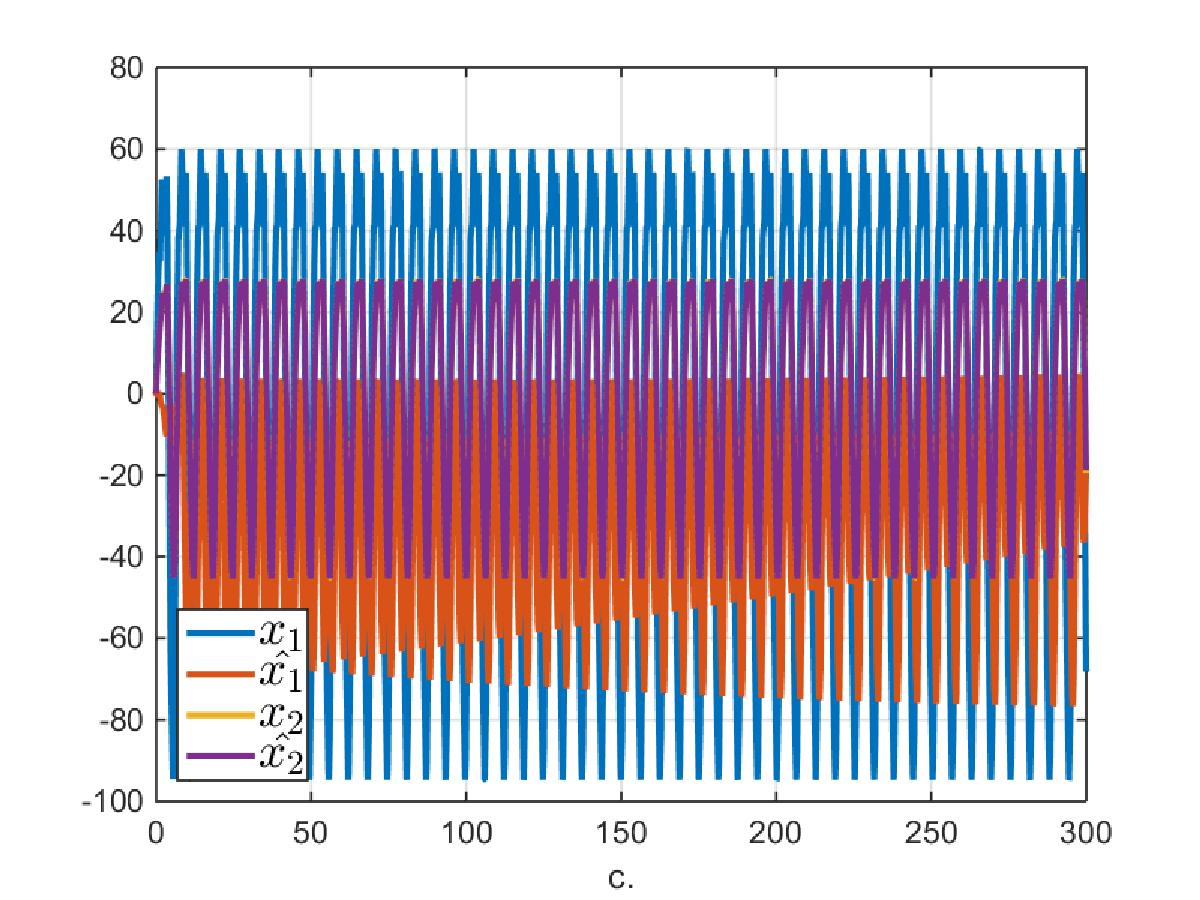
\includegraphics[width = 0.7\textwidth]{modeling62-x.jpg}
%	\caption{Переменные состояния} 
%	\label{modeling62-x}
%\end{figure}

%Тест привет

	
\end{document}